The filter design process is documented in this section, which includes determination of filter specifications, implementation and validation. As stated in section \ref{sec:filtervalg} a bandpass FIR filter of type I designed with use of a Kaiser window is wanted.\\
It is essential to note that the filter to be designed in this project is not an adaptive filter, meaning that the filter specifications will be chosen on behalf of a specific  input signal including a known noise signal. During final tests the filter is adapted to other signals only by changing the specifications for the cut off frequencies.

\subsection{Specifications of the filter} \label{sec:FIRspec} 
The purpose of this filter is to remove noise in the form of clapping hands from a signal representing a low E note. \\
Due to the frequency analysis of single tones described in section \ref{sec:single} the energy in the signal is located within a frequencyband from 75 Hz to 1000 Hz.  
By letting the cut off frequencies $f_c$ of the filter be respectively 75 Hz and 1000 Hz, this makes the passband of the filter.\\ 
According to section \ref{subsec:FIR} the Kaiser window can be determined from specifications of the allowed transition width $tw$ and peak approximation error $\delta$ of amplitude in pass and stop band.\\ 
By the frequency analysis of the specific noise showed by figure \ref{fig:clapping} it is seen that the frequencies of the noise are completely adjacent to the desired passband which verifies the need of a narrow transitionband. Though the narrower transitionband the higher order of filter is needed which gives more computations, hence it is not realistic to let the width of the transitionband go toward zero.  \\  
The maximum allowed width of the transitionband $tw$ and peak approximation error in amplitude $\delta$ determined as
\begin{align}
tw = 20 [Hz], \ \ \ \ \  \delta = 0.05 
\end{align}
The magnitude response of the ideal filter is sketched in figure \ref{fig:spec_Hd}, along with the boundaries for the real filter, provided by the defined specifications.      

\begin{figure}[H]
\centering
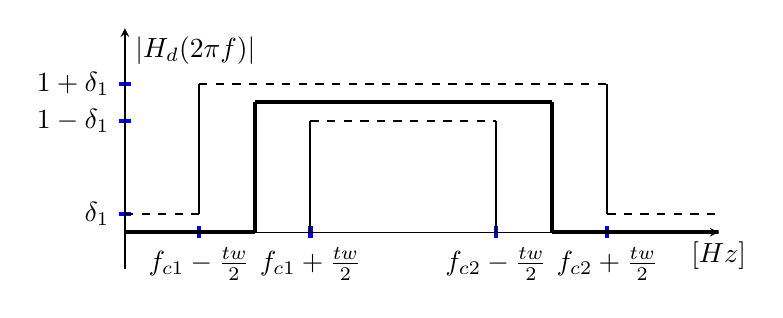
\begin{tikzpicture}[scale=1]
\begin{axis}[every tick/.style={blue, ultra thick}, 
scale=1.1,
unit vector ratio*=1 1 1,
axis lines = middle,
x label style={at={(current axis.right of origin)},anchor=north},
xlabel={$[Hz]$},
xtick={2,5,10,13},
xticklabels={$f_{c1}-\frac{tw}{2}$,$f_{c1}+\frac{tw}{2}$,$f_{c2}-\frac{tw}{2}$,$f_{c2}+\frac{tw}{2}$},
ytick={0.5,3,4},
yticklabels={$\delta_1$,$1-\delta_1$,$1+\delta_1$},
xmin=0,
xmax=16,
ymin=-1,
ymax=5.5]
\node at (axis cs:1.9,4.9) {$|H_d(2\pi f)|$};
\draw[line width=0.5mm](axis cs:0,0)--(axis cs:3.5,0);
\draw[line width=0.5mm](axis cs:3.5,0)--(axis cs:3.5,3.5);
\draw[line width=0.5mm](axis cs:3.5,3.5)--(axis cs:11.5,3.5);
\draw[line width=0.5mm](axis cs:11.5,3.5)--(axis cs:11.5,0);
\draw[line width=0.5mm](axis cs:11.5,0)--(axis cs:16,0);
\draw[line width=0.25mm, dashed](axis cs:0,0.5)--(axis cs:2,0.5);
\draw[line width=0.25mm, dashed](axis cs:13,0.5)--(axis cs:16,0.5);
\draw[line width=0.25mm, dashed](axis cs:5,3)--(axis cs:10,3);
\draw[line width=0.25mm, dashed](axis cs:2,4)--(axis cs:13,4);
\draw[line width=0.25mm](axis cs:2,0.5)--(axis cs:2,4);
\draw[line width=0.25mm](axis cs:5,0)--(axis cs:5,3);
\draw[line width=0.25mm](axis cs:10,0)--(axis cs:10,3);
\draw[line width=0.25mm](axis cs:13,4)--(axis cs:13,0.5);
%\draw[line width=0.5mm](axis cs:4,0.5)--(axis cs:7,0.5);
%\node at (axis cs:1,1.5) {Passband};
%\node at (axis cs:3,1.5) {Transition};
%\node at (axis cs:5.0,1.5) {Stopband};
\end{axis}
\end{tikzpicture}
\caption{Amplitude response of ideal filter within the boundaries for the amplitude response of the realizable filter, given by the defined specifications.}
\label{fig:spec_Hd}
\end{figure}

\subsection{Implementation of the filter}
The implementation of the filter basically follows algorithm \ref{alg:FIR}. The ideal impulse response is defined as the inverse Fourier transformation of the ideal filter specified on figure \ref{fig:spec_Hd}. For derivation of the ideal impulse response of a bandpass filter consult appendix \ref{appC}. Figure \ref{fig:freq_filt1} illustrates a plot of the amplitude response corresponding to the filter in the frequency domain. At \ref{fig:freq_filt2} illustrate a close up view of the left transition band, showing the ripples at in stop- and passband  the boundaries from the specifications are marked by the green lines. It is seen that the specifications are fulfilled.        
\begin{figure}[h]
\centering
\begin{subfigure}{0.49\textwidth}
\centering
\includegraphics[width=\textwidth]{figures/filtertest/freq_response1.pdf}
\caption{}
\label{fig:freq_filt1}
\end{subfigure}
\begin{subfigure}{0.49\textwidth}
\centering
\includegraphics[width=\textwidth]{figures/filtertest/freq_response2.pdf}
\caption{}
\label{fig:freq_filt2}
\end{subfigure}
\caption{(a) Amplitude response of filter. (b) Close up amplitude response of filter, showing top and bottom of one transitionband.}
\label{fig:freq_filt}
\end{figure}


\begin{algorithm}[H]
\caption{Compute type I FIR filter}
\label{alg:FIR}
\begin{algorithmic}[1] 
\State $f_s= 44100$ \Comment {Sampling frequency}
\State $f_{t1} = 75/f_s$ \Comment {Normalized transition frequency $1$}
\State $f_{t2} = 1000/f_s$ \Comment {Normalized transition frequency $2$}
\State $\delta = 0.05$  \Comment {Max. amplitude error }
\State $f_{tw} =20/ f_s$  \Comment {Normalized transition width}
\\
\Procedure{Compute kaiser window,$w$}{}
\State $A=-20\log_{10}(\delta)$ \Comment{$21 \leq A \leq 50$}
\State $\beta = 0.5824(A-21)^{0.4} + 0.07886(A-21)$ \Comment {Shape parameter}
\State $M = (A-8)/(2.285 \cdot f_{tw}  2\pi)$ \Comment {Filter order, round to upper even int.}
\State $N = M+1$ \Comment {Length of filter}
	\For {each integer $i$ in length of $N$}
		\For {each integer $j$ in length of $M$}
			\State $ sum_n = + \ (\frac{1}{j!})^2 \left( \left( \frac{\beta}{2} \sqrt{\left(1 - \left( \frac{2*i}{N-1}\right) - 1\right)^2}\right)^{2j}\right)$
			\State $ sum_d = + \ (\frac{1}{j!})^2 \left( \frac{\beta}{2}\right)^{j2}$
		\EndFor
		\State $w[i]=\frac{sum_n}{sum_d}$
	\EndFor
	\State Return $w$, $M$
\EndProcedure
\\
\Procedure{Compute ideal impulse response,$h_d$}{}
    \For {each integer $i$ in $h_d$}
        \If {$i == \frac{M}{2}$}
        		\State $h_d[i] = 2(f_{t2} - f_{t1})$
        	\Else 
        		\State  $h_d[i] = \frac{1}{ (\pi (i - \frac{M}{2}))}(\sin(f_{t2} 2 \pi (i - \frac{M}{2})) - (\sin(f_{t1} 2 \pi (i - \frac{M}{2}))))$ 
        	\EndIf 
	\EndFor
	\State Return $h_d$
\EndProcedure
\\
\Procedure{Compute impulse response, $h$}{}
	\State Return $h = h_d \cdot w$ \Comment{Windowed impulse response}
\EndProcedure


\end{algorithmic}
\end{algorithm}

\subsection{Validation of the filter}
The implemented filter is tested according to the test specifications described in section \ref{sec:testspec}. Figure \ref{fig:SIGNAL} show the frequency spectrum of the single low E note with additive noise in form of a beat of hands clapping. Figure \ref{fig:filt_SIGNAL} show the filtered signal. Note that the frequency spectrum are only showed from 0 to approximately 2200 $[Hz]$.  

\begin{figure}[H]
\centering
\begin{subfigure}{0.49\textwidth}
\centering
\includegraphics[width=\textwidth]{figures/filtertest/SIGNAL.pdf}
\caption{}
\label{fig:SIGNAL}
\end{subfigure}
\begin{subfigure}{0.49\textwidth}
\centering
\includegraphics[width=\textwidth]{figures/filtertest/filt_SIGNAL.pdf}
\caption{}
\label{fig:filt_SIGNAL}
\end{subfigure}
\caption{(a) Frequency spectrum of signal with noise (b) frequency spectrum of filtered signal}
\label{fig:test_res}
\end{figure}
As described in the specifications the filter is designed to remove all frequencies outside the frequency band from 75 Hz to 1000 Hz. It is seen by comparing figure \ref{fig:SIGNAL} and figure \ref{fig:filt_SIGNAL} that the frequencies outside the pass band appears to be zero and that the amplitudes of the remaining frequencies are appropriately the same. \\
By this the designed filter of order 2766 fulfil the specifications.\\
On behalf of this test it is assumed that by changing the cut off frequencies the filter can be modified to fit other music signals.  